\documentclass{article}

% Language setting
\usepackage[english]{babel}

% Set page size and margins
% Replace `letterpaper' with `a4paper' for UK/EU standard size
\usepackage[letterpaper,top=2cm,bottom=2cm,left=3cm,right=3cm,marginparwidth=1.75cm]{geometry}

% Useful packages
\usepackage{amsmath}
% --- Code listings ---
\usepackage{listings}
\usepackage{xcolor}
\definecolor{codegreen}{rgb}{0,0.6,0}
\definecolor{codegray}{rgb}{0.5,0.5,0.5}
\definecolor{codepurple}{rgb}{0.58,0,0.82}
\definecolor{backcolour}{rgb}{0.95,0.95,0.92}

\lstdefinestyle{mystyle}{
    backgroundcolor=\color{backcolour},   
    commentstyle=\color{codegreen},
    keywordstyle=\color{magenta},
    numberstyle=\tiny\color{codegray},
    stringstyle=\color{codepurple},
    basicstyle=\ttfamily\footnotesize,
    breakatwhitespace=false,         
    breaklines=true,                 
    captionpos=b,                    
    keepspaces=true,                 
    numbers=left,                    
    numbersep=5pt,                  
    showspaces=false,                
    showstringspaces=false,
    showtabs=false,                  
    tabsize=2
}

\lstset{style=mystyle}
% --- End Code Listings
\usepackage{graphicx}
\usepackage{float}
\usepackage{caption}
\captionsetup{labelformat=empty} 
% \usepackage{subcaption}
\usepackage[colorlinks=true, allcolors=blue]{hyperref}
\graphicspath{{./figures/}}

\title{ECE 637 Lab - Colorimetry}
\author{Colin Braun}

\begin{document}
\maketitle

\stepcounter{section}
\section{Plotting Color Matching Functions and Illuminants}
\begin{figure}[H]
    \centering
    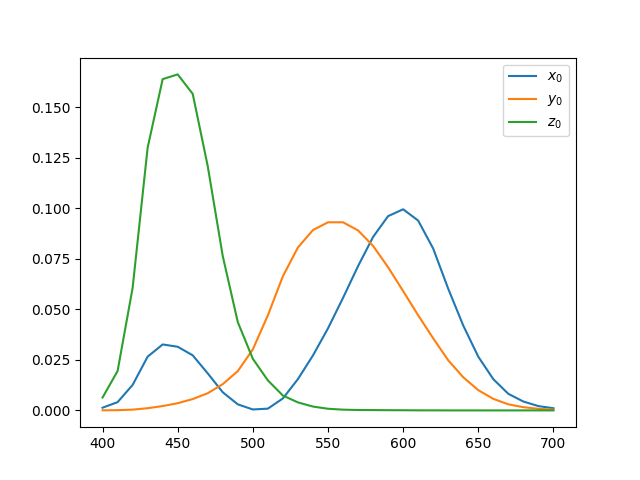
\includegraphics[width=1\textwidth]{../2-x0-y0-z0.png}
\end{figure}
\begin{figure}[H]
    \centering
    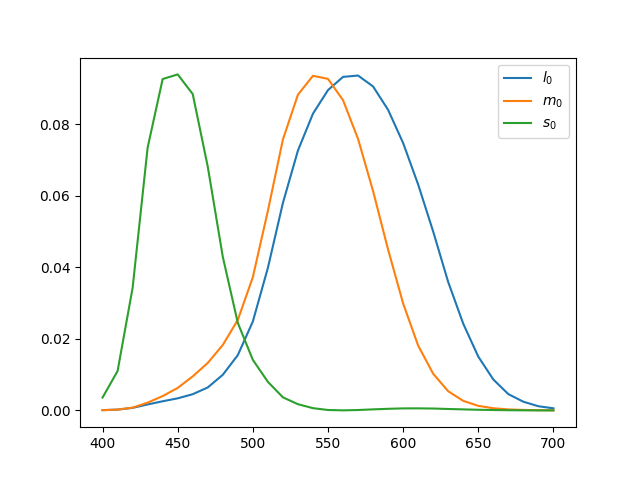
\includegraphics[width=1\textwidth]{../2-l0-m0-s0.png}
\end{figure}
\begin{figure}[H]
    \centering
    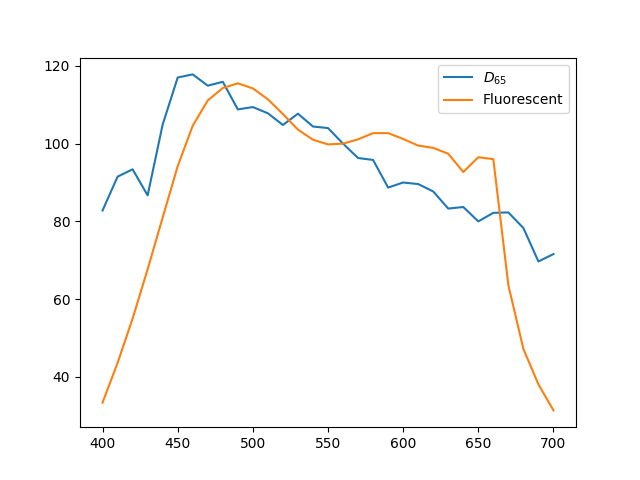
\includegraphics[width=1\textwidth]{../2-d65-and-fluorescent-illuminants.png}
\end{figure}

\section{Chromaticity Diagrams}
\begin{figure}[H]
    \centering
    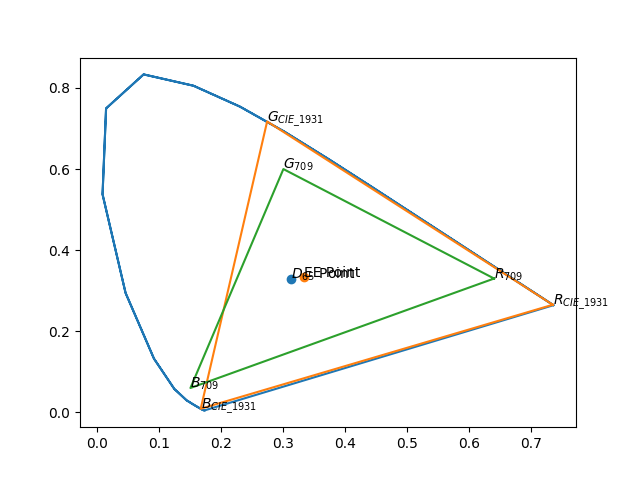
\includegraphics[width=1\textwidth]{../3-chromaticities-pure-source.png}
\end{figure}

\section{Rendering an Image from Illuminant, Reflectance, and Color Matching Functions}

The matrix $M_{709\_D65}$:
\begin{equation*}
\begin{bmatrix}
  3.24096994 & -1.53738318 & -0.49861076\\
  -0.96924364 & 1.8759675 & 0.04155506\\
  0.05563008 & -0.20397696 & 1.05697151\\
\end{bmatrix}
\end{equation*}

\begin{figure}[H]
    \centering
    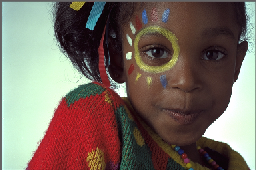
\includegraphics[width=1\textwidth]{../4-d65-illum1.png}
    \caption{The $D_{65}$ light source}
\end{figure}
\begin{figure}[H]
    \centering
    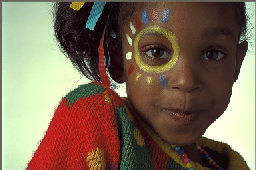
\includegraphics[width=1\textwidth]{../4-d65-illum2.png}
    \caption{The fluorescent light source}
\end{figure}

\pagebreak
\noindent
\textbf{Qualitiative description of the differences between the two images:}
The $D_{65}$ light source accentuates the blue more than the fluorescent light. The fluorescent light gives off a bit of a warmer feel than the $D_{65}$ light source.

\section{Color Chromaticity Diagram}
\begin{figure}[H]
    \centering
    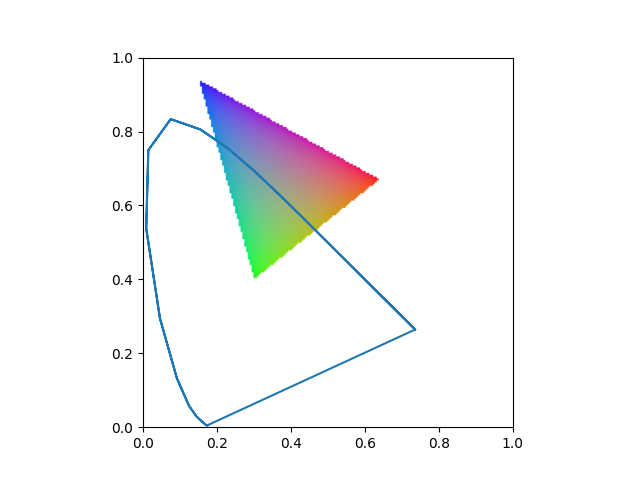
\includegraphics[width=1\textwidth]{../5-outlined-chromaticity-plot.png}
\end{figure}

\end{document}
